%%%%%%%%%%%%%%%%%%%%%%%%%%%%%%%%%%%%%%%%%%%%%%%%%%%%%%%%%%%%
\documentclass[a4paper,11pt,oneside]{article}
\usepackage[a4paper,vmargin={1.5cm,1.5cm},width=16cm]{geometry}
\usepackage[style=verbose-inote,doi=false,sortcites=true,block=space,backend=bibtex]{biblatex}
\usepackage[utf8]{inputenc}
\usepackage{textcomp}
\usepackage[english]{babel}
\usepackage{microtype}
\usepackage{lmodern}
\usepackage{graphicx}
\usepackage{fancyhdr}
\usepackage{booktabs}
\usepackage{eurosym}
\usepackage{mathptmx}
\usepackage[T1]{fontenc}
\usepackage{hyperref}
%% Added to help mimic structure.
\usepackage{tcolorbox}
\usepackage{soul}
\usepackage{color}
\usepackage{lastpage}

%%% HEADER
\setlength{\headheight}{1cm}
%\setlength{\headwidth}{20cm}
\setlength{\headsep}{0.5cm}
\pagestyle{fancyplain}
\fancyheadoffset[HR,HL]{2cm}
\fancyhf{}
\lhead{\raisebox{-0.4\height}{
\includegraphics[height=0.9cm,keepaspectratio=true]{img/miniLogo}}}
\rhead{\fancyplain{}{\fontsize{10}{12} \selectfont \textbf{\underline{MEMORIA CIENT\'IFICO-T\'ECNICA DE PROYECTOS de I+D+I PARA J\'OVENES INVESTIGADORES}}}}
\cfoot{\thepage\, / parte A}
\renewcommand{\headrulewidth}{0pt} % remove lines
\renewcommand{\footrulewidth}{0pt}


%%%%%%%%%%%%%%%%%%%%%%%%%%%%%%%%%%%%%%%%%%%%%%%%%%%%%%%%%%%%
%% Hack to make math formulas bold in section titles
\makeatletter
\DeclareRobustCommand*{\bfseries}{%
  \not@math@alphabet\bfseries\mathbf
  \fontseries\bfdefault\selectfont
  \boldmath
}
\makeatother

%%%%%%%%%%%%%%%%%%%%%%%%%%%%%%%%%%%%%%%%%%%%%%%%%%%%%%%%%%%%
\def\thesection{\bf \textsf{\alph{section}}}

\bibliography{biblio}

\begin{document}
% BB
\newcommand{\bb}{\ensuremath{\beta\beta}}
% BB0NU
\newcommand{\bbonu}{\ensuremath{\beta\beta0\nu}}
% BB2NU
\newcommand{\bbtnu}{\ensuremath{\beta\beta2\nu}}
% NME
\newcommand{\Monu}{\ensuremath{\Big|M_{0\nu}\Big|}}
\newcommand{\Mtnu}{\ensuremath{\Big|M_{2\nu}\Big|}}
% PHASE-SPACE FACTOR
\newcommand{\Gonu}{\ensuremath{G_{0\nu}(\Qbb, Z)}}
\newcommand{\Gtnu}{\ensuremath{G_{2\nu}(\Qbb, Z)}}

% mbb
\newcommand{\mbb}{\ensuremath{m_{\beta\beta}}}
\newcommand{\kgy}{\ensuremath{\rm kg \cdot y}}
\newcommand{\ckky}{\ensuremath{\rm counts/(keV \cdot kg \cdot y)}}
\newcommand{\mbba}{\ensuremath{m_{\beta\beta}^a}}
\newcommand{\mbbb}{\ensuremath{m_{\beta\beta}^b}}
\newcommand{\mbbt}{\ensuremath{m_{\beta\beta}^t}}
\newcommand{\nbb}{\ensuremath{N_{\beta\beta^{0\nu}}}}

% Qbb
\newcommand{\Qbb}{\ensuremath{Q_{\beta\beta}}}

% Tonu
\newcommand{\Tonu}{\ensuremath{T_{1/2}^{0\nu}}}

% Tonu
\newcommand{\Ttnu}{\ensuremath{T_{1/2}^{2\nu}}}

% Xe-136
\newcommand{\Xe}{\ensuremath{^{136}}Xe}

% 2S
\newcommand{\TwoS}{\ensuremath{^{2}S_{1/2}}}

\newcommand{\TwoP}{\ensuremath{^{2}P_{1/2}}}

\newcommand{\TwoD}{\ensuremath{^{2}D_{3/2}}}


% Xe-136
\newcommand{\CS}{\ensuremath{^{137}}Cs}

% Xe-136
\newcommand{\NA}{\ensuremath{^{22}}Na}


% Bi-214
\newcommand{\Bi}{\ensuremath{^{214}}Bi}

% Tl-208
\newcommand{\Tl}{\ensuremath{^{208}}Tl}

% Pb-208
\newcommand{\Pb}{\ensuremath{^{208}}Pb}
% Pb-208
\newcommand{\PBD}{\ensuremath{^{210}}Pb}

% Po-214
\newcommand{\Po}{\ensuremath{^{214}}Po}

% bru
\newcommand{\bru}{cts/(keV$\cdot$kg$\cdot$y)}
\newcommand{\HPXE}{\sc{HPXe}\rm}
\newcommand{\BATA}{\sc{BaTa}\rm}

% Saltos de carro en tablas
\newcommand{\minitab}[2][l]{\begin{tabular}{#1}#2\end{tabular}}

\newcommand{\thedraft}{0.1.1}% version for referees

\newcommand{\MO}{\ensuremath{{}^{100}{\rm Mo}}}
\newcommand{\SE}{\ensuremath{{}^{82}{\rm Se}}}
\newcommand{\ZR}{\ensuremath{{}^{96}{\rm Zr}}}
\newcommand{\KR}{\ensuremath{{}^{82}{\rm Kr}}}
\newcommand{\ND}{\ensuremath{{}^{150}{\rm Nd}}}
\newcommand{\XE}{\ensuremath{{}^{136}\rm Xe}}
\newcommand{\GE}{\ensuremath{{}^{76}\rm Ge}}
\newcommand{\GES}{\ensuremath{{}^{68}\rm Ge}}
\newcommand{\TE}{\ensuremath{{}^{128}\rm Te}}
\newcommand{\TEX}{\ensuremath{{}^{130}\rm Te}}
\newcommand{\TL}{\ensuremath{{}^{208}\rm{Tl}}}
\newcommand{\CA}{\ensuremath{{}^{48}\rm Ca}}
\newcommand{\CO}{\ensuremath{{}^{60}\rm Co}}
\newcommand{\PO}{\ensuremath{{}^{214\rm Po}}}
\newcommand{\U}{\ensuremath{{}^{235}\rm U}}
\newcommand{\CT}{\ensuremath{{}^{10}\rm C}}
\newcommand{\BE}{\ensuremath{{}^{11}\rm Be}}
\newcommand{\BO}{\ensuremath{{}^{8}\rm Be}}
\newcommand{\UDTO}{\ensuremath{{}^{238}\rm U}}
\newcommand{\CD}{\ensuremath{^{116}{\rm Cd}}}
\newcommand{\THO}{\ensuremath{{}^{232}{\rm Th}}}
\newcommand{\BI}{\ensuremath{{}^{214}}Bi}


\begin{tcolorbox}[colback=white,arc=0pt,outer arc=0pt,colframe=black,boxrule=0.6pt]
  \begin{center}
    Convocatoria 2014\\
    Proyectos de I+D+I para j\'ovenes investigadores sin vinculaci\'on o con vinculaci\'on temporal\\
    Direcci\'on General de Investigaci\'on Cient\'ifica y T\'ecnica\\
    Subdirecci\'on General de Proyectos de Investigaci\'on
  \end{center}
\end{tcolorbox}
\begin{tcolorbox}[colback=yellow,arc=0pt,outer arc=0pt,colframe=black,boxrule=0.6pt,left=0mm,right=0mm]
  \begin{center}
    AVISO IMPORTANTE\\
  \end{center}
    En virtud del art\'iculo 11 de la convocatoria \ul{\textbf{NO SE ACEPTAR\'AN NI SER\'AN SUBSABABLES MEMORIAS CIENT\'IFICO-T\'ECNICAS}} que no se presenten en este formato.\\
    \\
    \textbf{Lea detenidamente las instrucciones que figuran al final de este documento para rellenar correctamente la memoria cient\'ifico-t\'ecnica.}
    \\
  %\end{center}
\end{tcolorbox}
\vspace{3pt}
\begin{tcolorbox}[colback=yellow,arc=0pt,outer arc=0pt,colframe=black,boxrule=0.6pt,left=0mm]
  \textbf{Parte A: RESUMEN DE LA PROPUESTA/SUMMARY OF THE PROPOSAL}
\end{tcolorbox}

\vspace{12pt}

\noindent\textbf{INVESTIGADOR PRINCIPAL/Principal investigator} (Nombre y apellidos): Andrew Brian Laing\\
\vspace{12pt}

\noindent\textbf{INVESTIGADOR TUTOR/Tutor} (Nombre y apellidos): Juan Jos\'e G\'omez Cadenas\\
\vspace{24pt}

\noindent\textbf{T\'ITULO DEL PROYECTO:}\\
\textbf{ACR\'ONIMO:}\\
\textbf{RESUMEN} {\color{blue}{M\'aximo 3500 caracteres (incluyendo espacios en blanco):}}
\vspace{12pt}

\noindent\textbf{PALABRAS CLAVE:}\\
\vspace{12pt}

\noindent\textbf{TITLE OF THE PROJECT:}\\
\textbf{ACRONYM:}\\
\textbf{SUMMARY} {\color{blue}{Maximum 3500 characters (including spaces):}}
\vspace{12pt}

\noindent\textbf{KEY WORDS:}\\
\vspace{12pt}

\newpage
\setcounter{page}{1}
\cfoot{\fancyplain{}{\thepage\, / parte B}}

\begin{tcolorbox}[colback=yellow,arc=0pt,outer arc=0pt,colframe=black,boxrule=0.6pt,left=0mm]
  \textbf{Parte B: INFORMAC\'ON ESPEC\'IFICA DEL INVESTIGADOR TUTOR}
\end{tcolorbox}

\textbf{FINANCIACI\'ON P\'UBLICA Y PRIVADA (PROYECTOS Y/O CONTRATOS DE I+D+I) DEL INVESTIGADOR TUTOR} (repita la secuencia tantas veces como se precise hasta un máximo de 10 proyectos y/o contratos)

\begin{enumerate}
\item Researcher from the research team who participates in the grant: Juan Jos\'e G\'omez Cadenas.
  \begin{itemize}
  \item[] Grant reference: ERC. Advanced Grant 339787-NEXT 
  \item[] Title:  NEXT.
  \item[] Principal investigator: Juan Jos\'e G\'omez Cadenas
  \item[] Funding Agency: European Research Council (ERC)
  \item[] Duration: 01/02/2014 -- 01/02/2018
  \item[] Grant value: 2.8 M\euro
  \item[] Relation with this project: Same topic
  \item[] Project status: Granted
  \end{itemize}
\item Researcher from the research team who participates in the grant: Juan Jos\'e G\'omez Cadenas.
  \begin{itemize}
  \item[] Grant reference: CSD2008-00037 
  \item[] Title:  Canfranc Underground Physics (CUP)
  \item[] Principal investigator: Concepci\'on Gonz\'alez Garc\'ia 
  \item[] Funding Agency: Ministerio de Educaci\'on y Ciencia
  \item[] Duration: 01/09/2014 -- 31/12/2015
  \item[] Grant value: 5.0 M\euro
  \item[] Relation with this project: Same topic
  \item[] Project status: Granted
  \end{itemize}
\item Researcher from the research team who participates in the grant: Juan Jos\'e G\'omez Cadenas.
  \begin{itemize}
  \item[] Grant reference: FIS2012-37947-C04-01 
  \item[] Title:  Coordination of NEXT Project
  \item[] Principal investigator: Juan Jos\'e G\'omez Cadenas
  \item[] Funding Agency:  Ministerio de Econom\'ia y Competitividad
  \item[] Duration: 01/01/2013 -- 31/12/2014
  \item[] Grant value: 256000\euro
  \item[] Relation with this project: Same topic
  \item[] Project status: Granted
  \end{itemize}
\item Researcher from the research team who participates in the grant: Juan Jos\'e G\'omez Cadenas.
  \begin{itemize}
  \item[] Grant reference: FPA2009-13697-C04-04 
  \item[] Title:  Física Experimental de Neutrinos en el IFIC / Experimental neutrino physics at IFIC 
  \item[] Principal investigator: Juan Jos\'e G\'omez Cadenas
  \item[] Funding Agency:  Ministerio de Educaci\'on y Ciencia, 
  \item[] Duration: 01/01/2010 -31/12/2012.
  \item[] Grant value: 534437\euro. 
  \item[] Relation with this project: Very related
  \item[] Project status: Granted
  \end{itemize}
\end{enumerate}

\newpage
\setcounter{page}{1}
\cfoot{\fancyplain{}{\thepage\, de \pageref{LastPage} / parte C}}

\begin{tcolorbox}[colback=yellow,arc=0pt,outer arc=0pt,colframe=black,boxrule=0.6pt,left=0mm]
  \textbf{Parte C: DOCUMENTO CIENT\'IFICO}
\end{tcolorbox}

\noindent\textbf{C.1. PROPUESTA CIENT\'IFICA}
\subsection*{The state of the art}
\subsubsection*{Introduction}
Neutrinos, unlike the other fermions of the Standard Model of particle physics, could be Majorana particles, that is, indistinguishable from their antiparticles. The existence of Majorana neutrinos would have profound implications in particle physics and cosmology. 

If neutrinos are Majorana particles, there must exist a new scale of physics (at a level inversely proportional to the neutrino masses) that characterises underlying dynamics beyond the Standard Model. The existence of such a new scale provides the simplest explanation of why neutrino masses are so much lighter than the charged fermions. Indeed,  understanding the new physics that underlies neutrino masses is one of the most important open questions in particle physics and it could have profound implications in our comprehension of the mechanism of symmetry breaking, the origin of mass, and the flavour problem. 

The existence of Majorana neutrinos would imply that lepton number is not conserved, which could be the origin of the matter-antimatter asymmetry observed in the Universe. The new physics related to neutrino masses could provide a new mechanism to generate the asymmetry called leptogenesis. Although the predictions are model dependent, two essential ingredients must be confirmed experimentally: 1) the violation of lepton number and 2) CP violation in the lepton sector. 

The only practical way to establish experimentally that neutrinos are their own antiparticles and that lepton number is not conserved is the detection of neutrinoless double beta decay (\bbonu). This is a hypothetical, very slow nuclear transition in which a nucleus with $Z$ protons decays into a nucleus with $Z+2$ protons and the same mass number $A$, emitting two electrons that carry essentially all the energy released (\Qbb). The process can occur if and only if neutrinos are Majorana particles.

%%%%%%%%%%%%%%%%%%%%%%%%%%%%%%%%%%%%%%%%%%%%%%%%%%%%%%%%%%%%
\subsubsection*{The experimental landscape}
The detectors used in double beta decay searches are designed to measure the energy of the radiation emitted by a \bb\ source. In the case of \bbonu, the sum of the kinetic energies of the two released electrons is fixed by the mass difference between the parent and the daughter nuclei: $Q_{\bb} \equiv M(Z,A)-M(Z+2,A)$. However, due to the finite energy resolution of any detector, \bbonu\ events are reconstructed within an energy region centered around \Qbb, typically following a gaussian distribution (Region of Interest or ROI). Other processes occurring in the detector can fall in the ROI, becoming a background and compromising the expected sensitivity. It follows that \bbonu\ experiments require {\bf excellent energy resolution}, and good {\bf suppression of potential backgrounds}.

All double beta decay experiments have to deal with an intrinsic background, i.e. the standard process of a double $\beta$-decay with the emission of two neutrinos (\bbtnu), that can only be suppressed by means of good energy resolution. Cosmogenic backgrounds can be suppressed by underground opperation and those from natural radioisotopes present in the materials of the detector and its surroundings by careful screening and selection of materials. {\bf Additional experimental signatures} that allow the distinction between signal and background can further improve the S/N have been a major area of development for the next generation of experiments. Several other factors such as {\bf detection efficiency} or the {\bf scalability to large masses} must be also taken into account during the design of a double beta decay experiment.
 
\subsubsection*{Recent results}
The status of the field has been reviewed recently by the project tutor\footcite{INSS2014}. Three current-generation experiments, with fiducial masses in the range of the 100 kg, have recently published the \bbonu\ search results. These are: GERDA, a high resolution calorimeter using \GE\ diodes; KamLAND-Zen, a low resolution, high-mass, self-shielding liquid scintillator calorimeter, with \XE\ dissolved in the scintillator; and EXO-200, a liquid xenon (LXe) TPC. All the experiments published negative results and, therefore, an upper limit on the halflife of the \bbonu\ decay (\Tonu). This limit can be translated into a limit on the \emph{effective Majorana mass} of the electron neutrino defined as:
\begin{equation}
\mbb = \Big| \sum_{i} U^{2}_{ei} \ m_{i} \Big| \, ,
\end{equation}
%
where $m_{i}$ are the neutrino mass eigenstates and $U_{ei}$ are elements of the neutrino mixing matrix. \mbb\ is related to \Tonu\ through the equation:
\begin{equation}
(T^{0\nu}_{1/2})^{-1} = G^{0\nu} \ \big|M^{0\nu}\big|^{2} \ \mbb^{2} \, .
\label{eq:Tonu}
\end{equation}

Here, $G^{0\nu}$ is an exactly-calculable phase-space integral for the emission of two electrons and $M^{0\nu}$ is the nuclear matrix element (NME) of the transition, which has to be evaluated theoretically. The uncertainty in the NME affects the value of \mbb\ which can be obtained from \Tonu.
 
{\bf GERDA} \footcite{Agostini:2013mzu} has a resolution of $\sim$0.2 \% FWHM around the \Qbb\ of \GE. The specific background rate in the ROI is $10^{-2}$ \ckky\ and the total exposure deployed 21.6 kg $\times$ yr. The experiment sets a limit $\Tonu > 2 \times 10^{25}$~yr, which translates to a range for \mbb\ of $[258-649]$~meV. The lowest value of \mbb\ corresponds to the IBM2 NME set, while the highest value corresponds to the ISM set.

{\bf EXO} \footcite{Albert:2014awa} achieves an energy resolution of 3.6\% FWHM at \Qbb, and a background rate of $ 4 \times 10^{-3}\ckky$. The total exposure used for the published result is 100 kg$\cdot$~yr. They have published a limit on the half-life of \bbonu\ in \XE\ of $T_{1/2}^{0\nu}(\XE) > 2 \times 10^{25}$~yr (assuming background only). The limit translates into a range for \mbb\ of $[125-352]$~meV.

{\bf KamLAND-Zen} \footcite{TheKamLAND-Zen:2014lma} compensates for a worse energy resolution of 10\% FWHM at \Qbb\ with a very small background rate of $\sim 4 \times 10^{-4}$ \ckky. After an exposure of 108.8 kg$\cdot$~yr, they obtain a limit  $T_{1/2}^{0\nu}(\XE) > 2.6 \times 10^{25}$~yr, which translates into a range for \mbb\ of $[110-309]$~meV.

 \subsubsection*{Potential for discovery}
 %%%%%%
%\begin{figure}
%\centering
%\includegraphics[width=0.75\textwidth]{img/SensiCRR.png}
%\caption{The allowed \mbb\ region, as a function of the sum of the neutrino masses, assuming that 
%$\sum m_i = 0.32$~eV. The blue lines mark the sensitivity of EXO and KamLAND-ZEN, the xenon-based detectors currently leading the field. The red line shows the sensitivity of NEXT after 3 years operation, which gives the experiment a sizeable chance of making a discovery.} 
%\label{fig.mbb}
%\end{figure}
%%%%%%
 Several analyses from recent cosmological results suggest that the sum of the masses of the three neutrinos could be $\sim$0.3~eV\footcite{PhysRevLett.112.051303}. The PI and collaborators have demonstrated that, in this case, if the neutrino is a Majorana particle, then, $\mbb \sim [20-150]$~ meV \footcite{GomezCadenas:2013ue}. In this scenario, the sensitivity of GERDA is outside the ``cosmologically relevant region'' (CRR), while both EXO-200 and KamLAND-Zen have already explored a significant fraction of CRR {\em for the most optimistic NME set} (in the most pessimistic NME they have not yet explored any part of the CRR). 
 
% Clearly, the experimental effort to determine if the neutrino is a Majorana particle, far from being completed is, rather, in its infancy. To establish unambiguously that the neutrino is (or not) a Majorana particle, even in this favourable scenario in which the sum of the neutrino masses is relatively high, experiments must be sensitive to $\mbb \sim 20$~meV, {\em even for the most pessimistic NME} set. On the other hand, a xenon experiment probing a $\Tonu >2.6 \times 10^{25}$~yr, has chances of making a discovery.
% 
 
%%%%%%%%%%%%%%%%%%%%%%%%%%%%%%%%%%%%%%%%%%%%%%%%%%%%%%%%%%%%
\subsubsection*{The NEXT experiment and its innovative concepts}
\begin{figure}
\centering
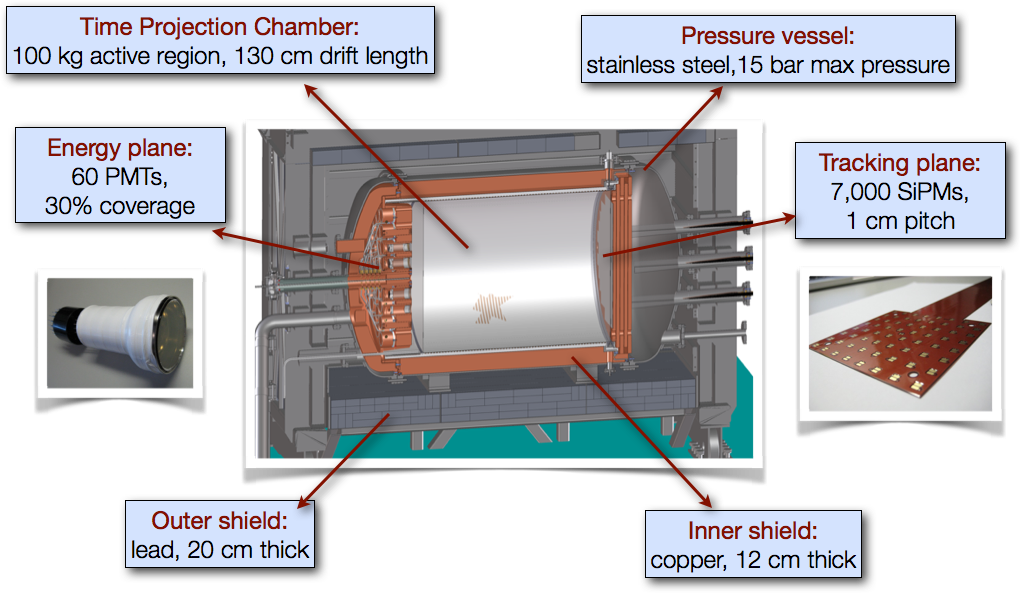
\includegraphics[width=0.9\textwidth]{img/NEXT.png}
\caption{\small A drawing of the NEXT-100 detector showing its main parts.  The pressure vessel (PV),  (130 cm inner diameter, 222 cm length, 1cm thick walls, with a total mass of 1\,200 kg) is made of a radio pure steel-titanium alloy.
The inner copper shield (ICS), is made of ultra-pure copper bars, 12 cm thick, with a total mass of 9\,000 kg.The electrical system includes the field cage, cathode, EL grids and HV penetrators.
The light tube is made of thin teflon sheets coated with TPB (a wavelength shifter). 
The energy plane is made of 60 PMTs housed in copper enclosures (cans).
The tracking plane is made of MPPCs arranged into dice boards (DB). 
}
\label{fig.NEXT100}
\end{figure}

The \emph{Neutrino Experiment with a Xenon TPC} (NEXT)\footnote{\href{http://next.ific.uv.es/}{http://next.ific.uv.es/}} will search for the \bbonu\ of \XE\ high-pressure gas (enriched to 91\%) using a time projection chamber (\HPXE). The advantages of the technology are: 
a) {\bf excellent energy resolution}, with an intrinsic limit of about 0.3\% FWHM at \Qbb, close to that of \GE\ detectors; b)
{\bf tracking capabilities} that provide a powerful topological signature to discriminate between signal (two electron tracks with a common vertex) and background (mostly, single electrons); c)
{\bf a fully active and homogeneous detector}, with no dead regions; d) {\bf scalability} of the technique to larger masses; %e) the possibility of exciting the barium ion produced in the xenon decay from the fundamental state \TwoS\ to the state \TwoP, using a ``blue'' laser (493.54 nm), and observing the ``red light'' emitted in the transition from \TwoP to \TwoD, thus ``tagging'' the presence of a barium atom in the xenon gas, which cannot be produced by any known background. 

The design of NEXT-100 (Figure \ref{fig.NEXT100}) is optimised for energy resolution by using proportional electroluminescent (EL) amplification of the ionisation signal. The detection process involves using the prompt scintillation light from the gas as start-of-event time, drifting the ionisation charge to the anode by means of an electric field ($\sim0.3$~kV~cm$^{-1}$ at 15 bar) where secondary EL scintillation will be produced in the region defined by two highly transparent meshes, between which there is a field of $\sim20$~kV~cm$^{-1}$ at 15~bar. The detection of EL light provides an energy measurement (in the energy plane, made of photomultipliers (PMTs), located behind the cathode) as well as providing tracking through its detection a few mm away from production at the anode plane, via a dense array of silicon photomultipliers called the \emph{tracking plane}.

\subsubsection*{The NEW detector}
\label{sec.new}
%%%%%%%%%%
\begin{figure}
\centering
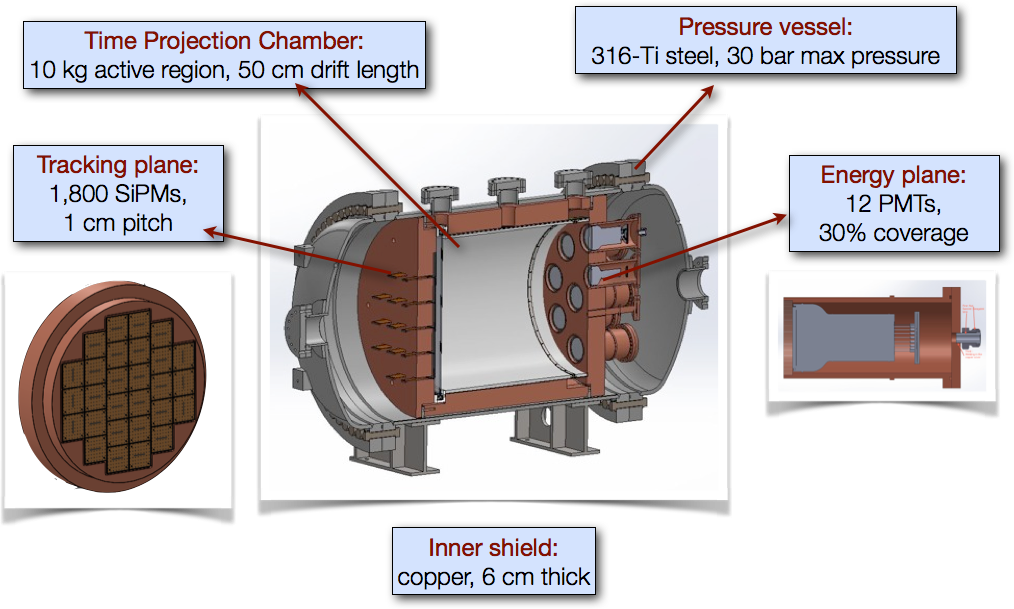
\includegraphics[height=9cm]{img/NEW.png}
\caption{The NEW apparatus.} \label{fig:NEW}
\end{figure}

The NEW (NEXT-WHITE) apparatus\footnote{The name honours the memory of the late Professor James White, one of the key scientists of the NEXT Collaboration.}, shown in Figure \ref{fig:NEW} is the first phase of the NEXT detector to operate underground. NEW 
%has a triple goal:
%
%\begin{enumerate}
%\item {\bf Technology}: it will validate the technological solutions adopted by NEXT-100.
%\item {\bf Radiopurity}: it will allow the NEXT collaboration an extra step in the implementation of a radiopure detector.
%\item {\bf Physics}: it will demonstrate with measurements of the \BI\ and \TL\ lines, as well as with the measurement of the \bbtnu\ spectrum, the physics capabilities of NEXT-100.
%\end{enumerate}
%
has a scale 1:2 in size (1:8 in mass) compared to NEXT-100. The energy plane contains 12 PMTs (20 \% of the 60 PMTs deployed by NEXT-100). The tracking plane technology consists of 30 Kapton Dice Boards (KDB) deploying 1800 SiPMs (also 20\% of the sensors). The field cage has a diameter of 50~cm and a length of 60~cm (the dimensions of the NEXT-100 field cage are roughly 1~m length and 1.2~m radius). 

NEW is a necessary step\footnote{As formally stated by the scientific committee of the LSC, who recommended its construction in 2013.} towards the construction of NEXT-100. It will validate the technological solutions adopted by the collaboration and, as discussed below, is essential in the definition of the project methodology. Furthermore, The NEXT background model is currently based on a sophisticated Monte Carlo simulation of all expected background sources in each part of the detector. NEW will allow the validation of the background model with data. 
%Last but not least, NEW operation will demonstrate with measurements of the \BI\ and \TL\ lines, as well as with the measurement of the \bbtnu\ spectrum, the physics capabilities of NEXT-100.

%Furthermore, the calibration of NEW with 
%sources of higher energy, will allow a precise study of the evolution of the resolution with the energy. 
%In particular it will be plausible to measure the resolution near \Qbb\ using a Thorium source, which provides 2.6 MeV gammas. Last, but not least, we intend to 
%reconstruct the spectrum of \bbtnu. Those events are topologically identical to signal events (\bbonu) and can be used to demonstrate with data the power of the topological signature. 
%
\subsubsection*{Discovery potential of NEXT-100}
The excellent resolution of NEXT (0.5 \% FWHM) and the combination of low radioactive budget and topological signature (which yields an expected background rate of $5 \times 10^{-4} \ckky$, will allow the NEXT-100 detector to reach a sensitivity to the \bbonu\ halflife of $\Tonu > 7 \times 10^{25}$~yr for a exposure of 300~kg$\times$yr. This translates to a range for \mbb\ of $[67-187]$~meV. Therefore NEXT-100 will have a substantial chance of making a discovery if the NME is sufficiently high.

\subsection*{Involvement of the PI in NEXT to date and its impact on the project}
\label{subSec:Past}
The PI of this project began his involvement in the experiment in October of 2012, first as a visiting researcher then as a contracted member of the IFIC group from March 2013. During his time as a memeber of the collaboration he has worked in various aspects of the experiment. 
\begin{figure}
  \centering
  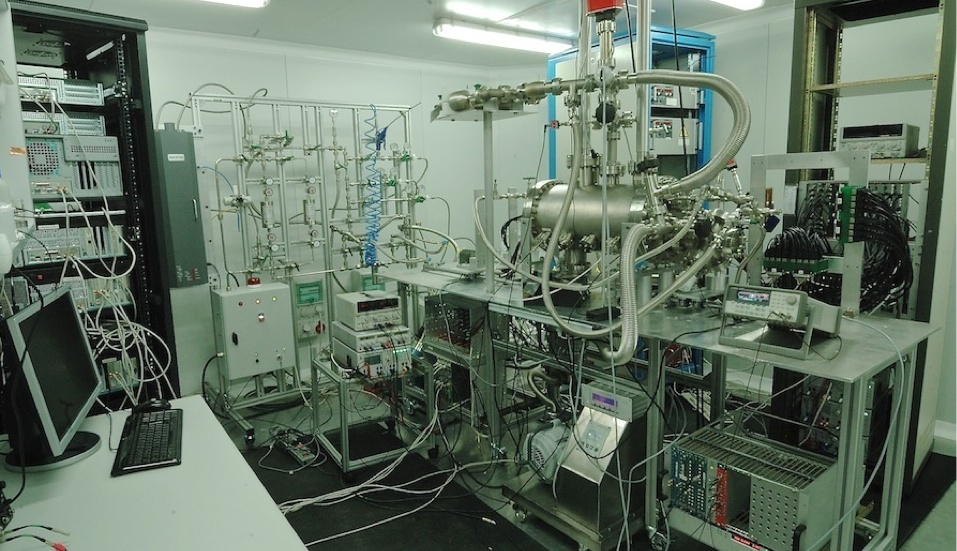
\includegraphics[width=0.7\textwidth]{img/DemoSetup.jpg}
  \caption{\small The NEXT-DEMO prototype setup at IFIC.} \label{fig.DEMO}
\end{figure}
%%%%%%%%%% 
A $\sim$1.5~kg natural xenon prototype of next (NEXT-DEMO, shown in figure~\ref{fig.DEMO}) has been taking data for the last two years at IFIC. NEXT-DEMO is  equipped with an energy plane made of 19 Hamamatsu R7378A PMTs and a tracking plane made of 256 Hamamatsu SiPMs. The detector has been operating successfully for more than two years and has demonstrated: (a) very good operational stability, with no leaks and very few sparks; (b) good energy resolution; (c) track reconstruction with PMTs and with SiPMs coated with TPB; (d) excellent electron drift lifetime, of the order of 20 ms. Its construction, commissioning and operation has been instrumental in the development of the required knowledge to design and build the NEXT detector.

The data taken over the course of the last two years has resulted in the publication of papers on the basic function and effect of wavelength shifting\footcite{Alvarez:2012xda}, the detection of alpha particles\footcite{Alvarez:2012hu}, improved resolution and basic tracking using SiPMs\footcite{Alvarez:2013gxa} and the use of Xe X-rays for characterisation and energy resolution improvement\footcite{Lorca:2014sra}. The PI has been a major author and internal editor in all of these papers with further papers currently being written. Currently, the data driven prediction of the energy resolution of NEXT at \Qbb\ is $\sim$0.7\% (see figure \ref{fig.ERES}).
%%%%% 
\begin{figure}
  \centering
  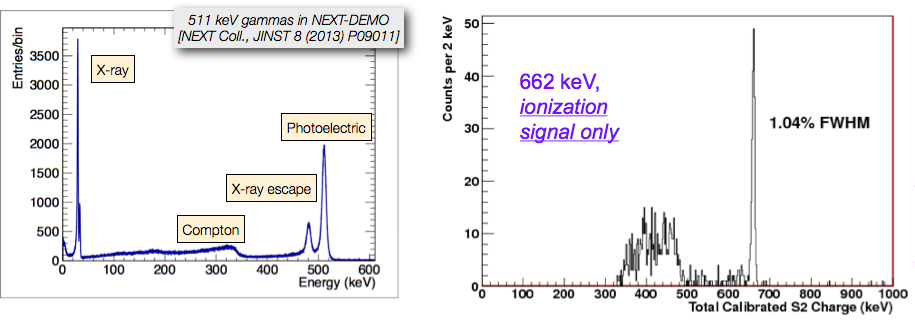
\includegraphics[width=0.8\textwidth]{img/EResolution.png}
  \caption{\small Left: the full energy spectrum measured for electrons of 511 keV in the DEMO detector. Right the spectrum near the photoelectric peak for 662 keV electrons in NEXT-DBDM. The resolution at 662 keV is 1\% FWHM (0.5\% FWHM at \Qbb). The resolution extrapolated from 511 keV is 0.7\%.}\label{fig.ERES}. 
\end{figure}
%%%% 

\subsubsection*{Run coordination for NEXT-DEMO data taking}
The PI has served as the run coordinator of these data runs organising a weekly run coordination meeting with all members of the group to decide calibration, maintenance and data scheduling. Additionally, he was responsable for the definition of shift and data monitoring duties for the members of the group and the scheduling of shifts and training for the newer members.

\subsubsection*{Detector calibration}
Calibration of the PMTs and SiPMs of NEXT is an important first step
in the commissioning of the detector. Using NEXT-DEMO the PI has been
involved in the improvement and standardisation of the basic
methodology for the calibration of the PMTs, work which will be
extended to NEW and NEXT-100. As seen in figure\ref{fig:cal}-\emph{left}, the low light
PMT spectra are fitted to a function which models the pedestal and a
number of related Gaussians representing the probability of detection
of one or multiple photoelectrons. Moreover, the PI suggested a backup
method for the calibration of the SiPMs in case of high electronic
noise (improving the calibration of certain channels and, thus, the
tracking plane as a whole) using the PTC
method\footcite{Janesick:2001}. This method determines the conversion
gain of the sensor by determining the gradient of a plot relating
variance and mean signal of the detection region
in which photon shot noise dominates (see figure \ref{fig:cal}-\emph{right}).
\begin{figure}
  \begin{center}
    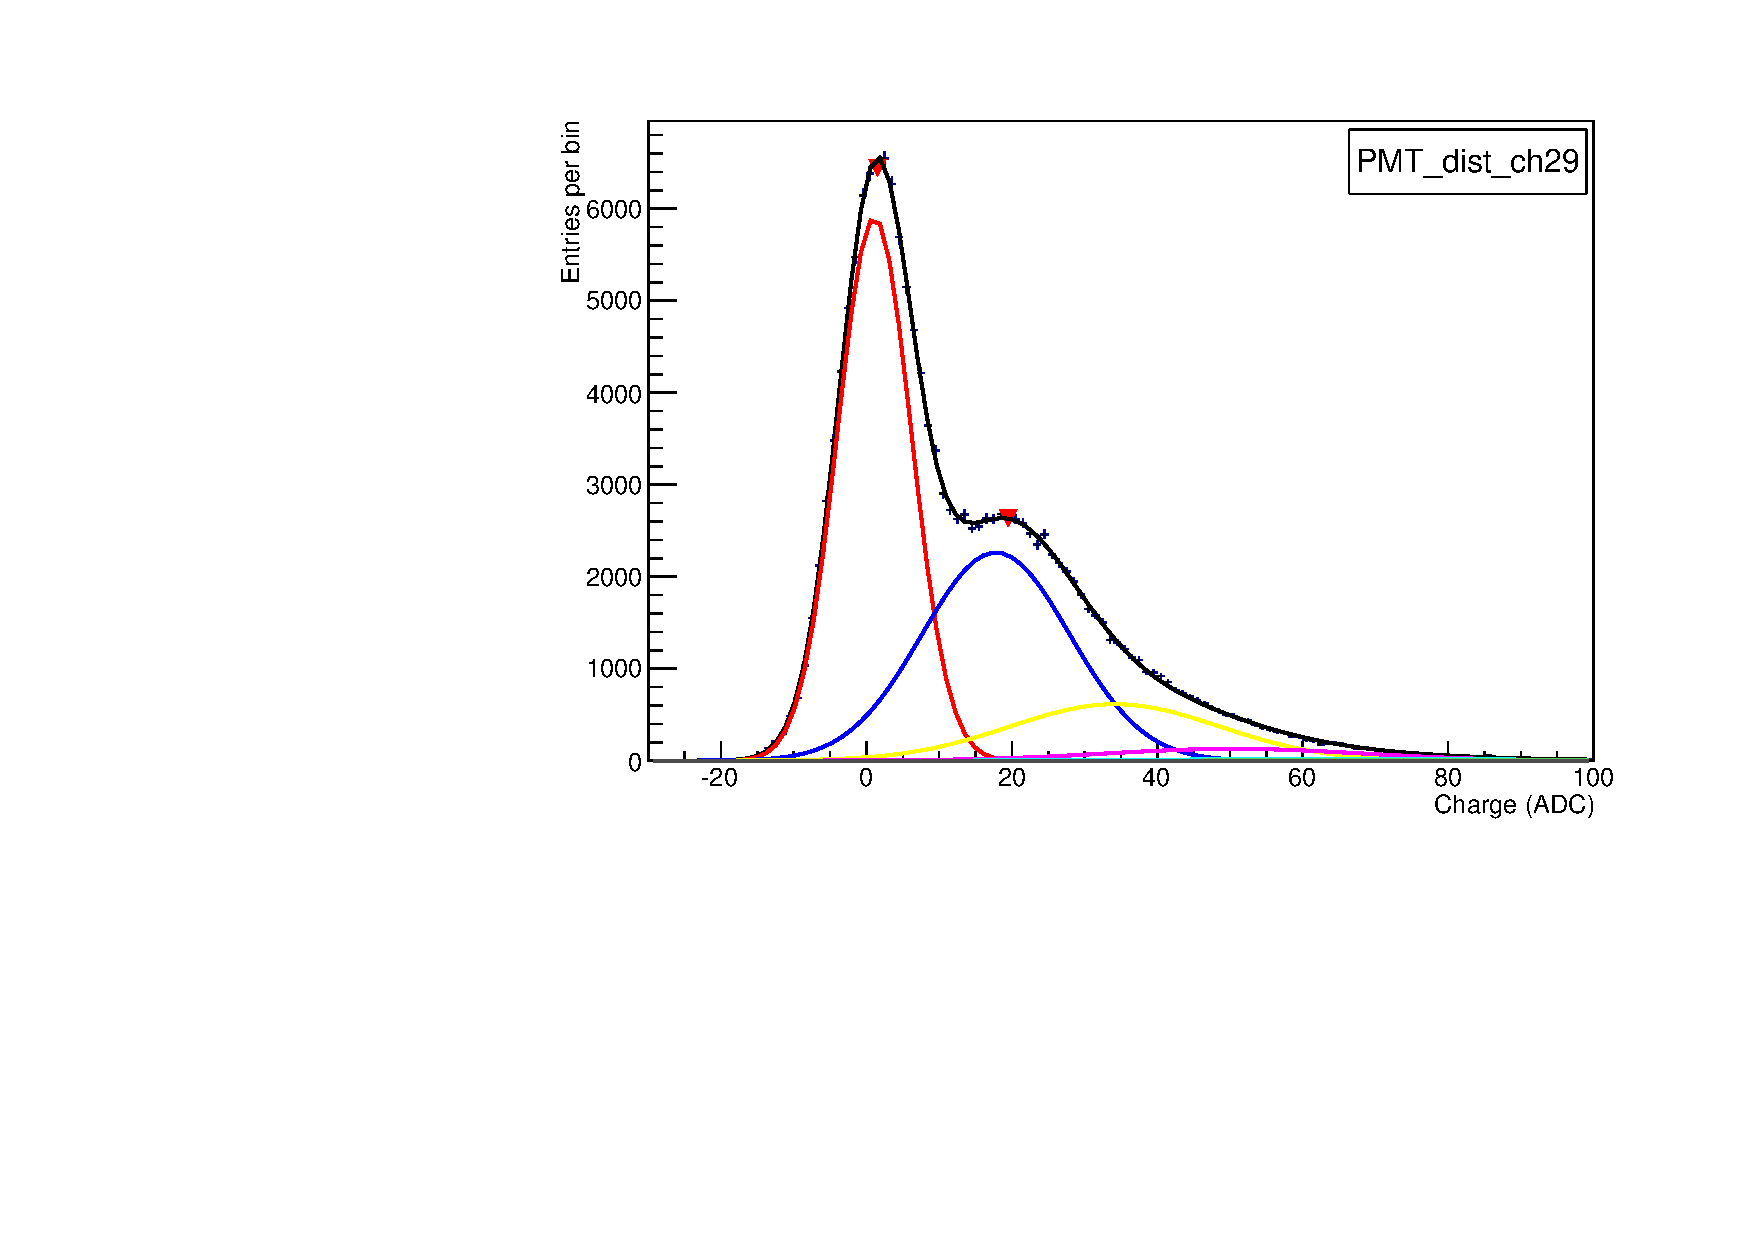
\includegraphics[width=0.45\textwidth]{img/pmtFitEx}
    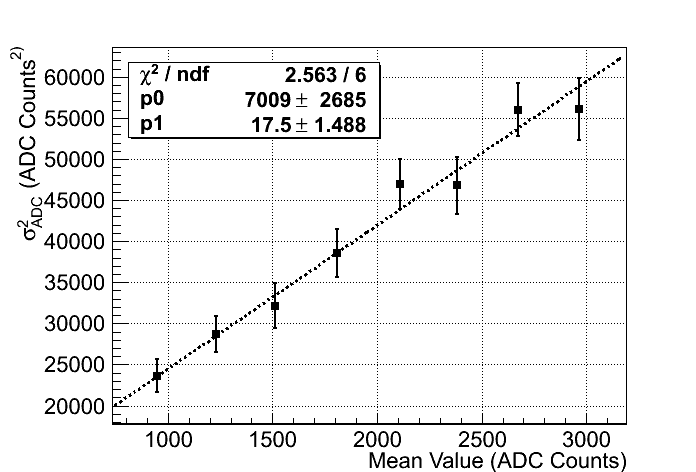
\includegraphics[width=0.45\textwidth]{img/Silinfit.png}
  \end{center}
  \caption{Sensor conversion gain extraction. (left) PMT response
    function, (right) a PTC curve for an example channel.}
  \label{fig:cal}
\end{figure}

\subsubsection*{Analysis of NEXT-DEMO data}
NEXT-DEMO data using atmospheric radiation as well as alpha particles
and gammas from radioactive sources has been recorded over the course
of the data taking runs mentioned above. The PI has been involved at
all levels of data processing and analysis. He has made improvements
to the data preprocessing algorithms particularly in the area of the
selection of SiPMs with signal and the exclusion of noisey
channels. In higher level analysis he has improved and developed a
series of cuts to further exlude events containing high noise levels,
possible sparks and particles of different types than those expected
in the run in question. He has also been active in the development of
the track reconstruciton algorithms currently considered the baseline
method for the experiment and using these algorithms has improved the
method of energy reconstruction by generalising the correction factors
to work with them. %Plot of some result been involved in?

\subsubsection*{Coordination of energy plane group for LSC based detectors}
As an additional coordination job, the PI has acted as coordinator of
the construction of the energy plane of NEW (and, ultimately, will
perform the same function for NEXT-100). Specifically, he has worked
to find appropriate optical coupling for the PMTs to their protective
sapphire windows and helped in the testing of said gel under
vacuum. Figure \ref{fig:gelRGA} shows a the results from a RGA measurement of
a sample of NyoGel OCK-451 showing little difference to the 'no
sample' measurement. Figure \ref{fig:gelPer} shows the improvement in light
collection efficiency achieved using this product to optically couple
a sapphire window to a PMT with the same window material as those to be
used in NEW/NEXT-100. He has also been responsible for collating the
costs and outstanding issues related to the radiopurity, cleaning and
construction for all mechanical and
electronic components of the energy plane.
\begin{figure}
  \begin{center}
    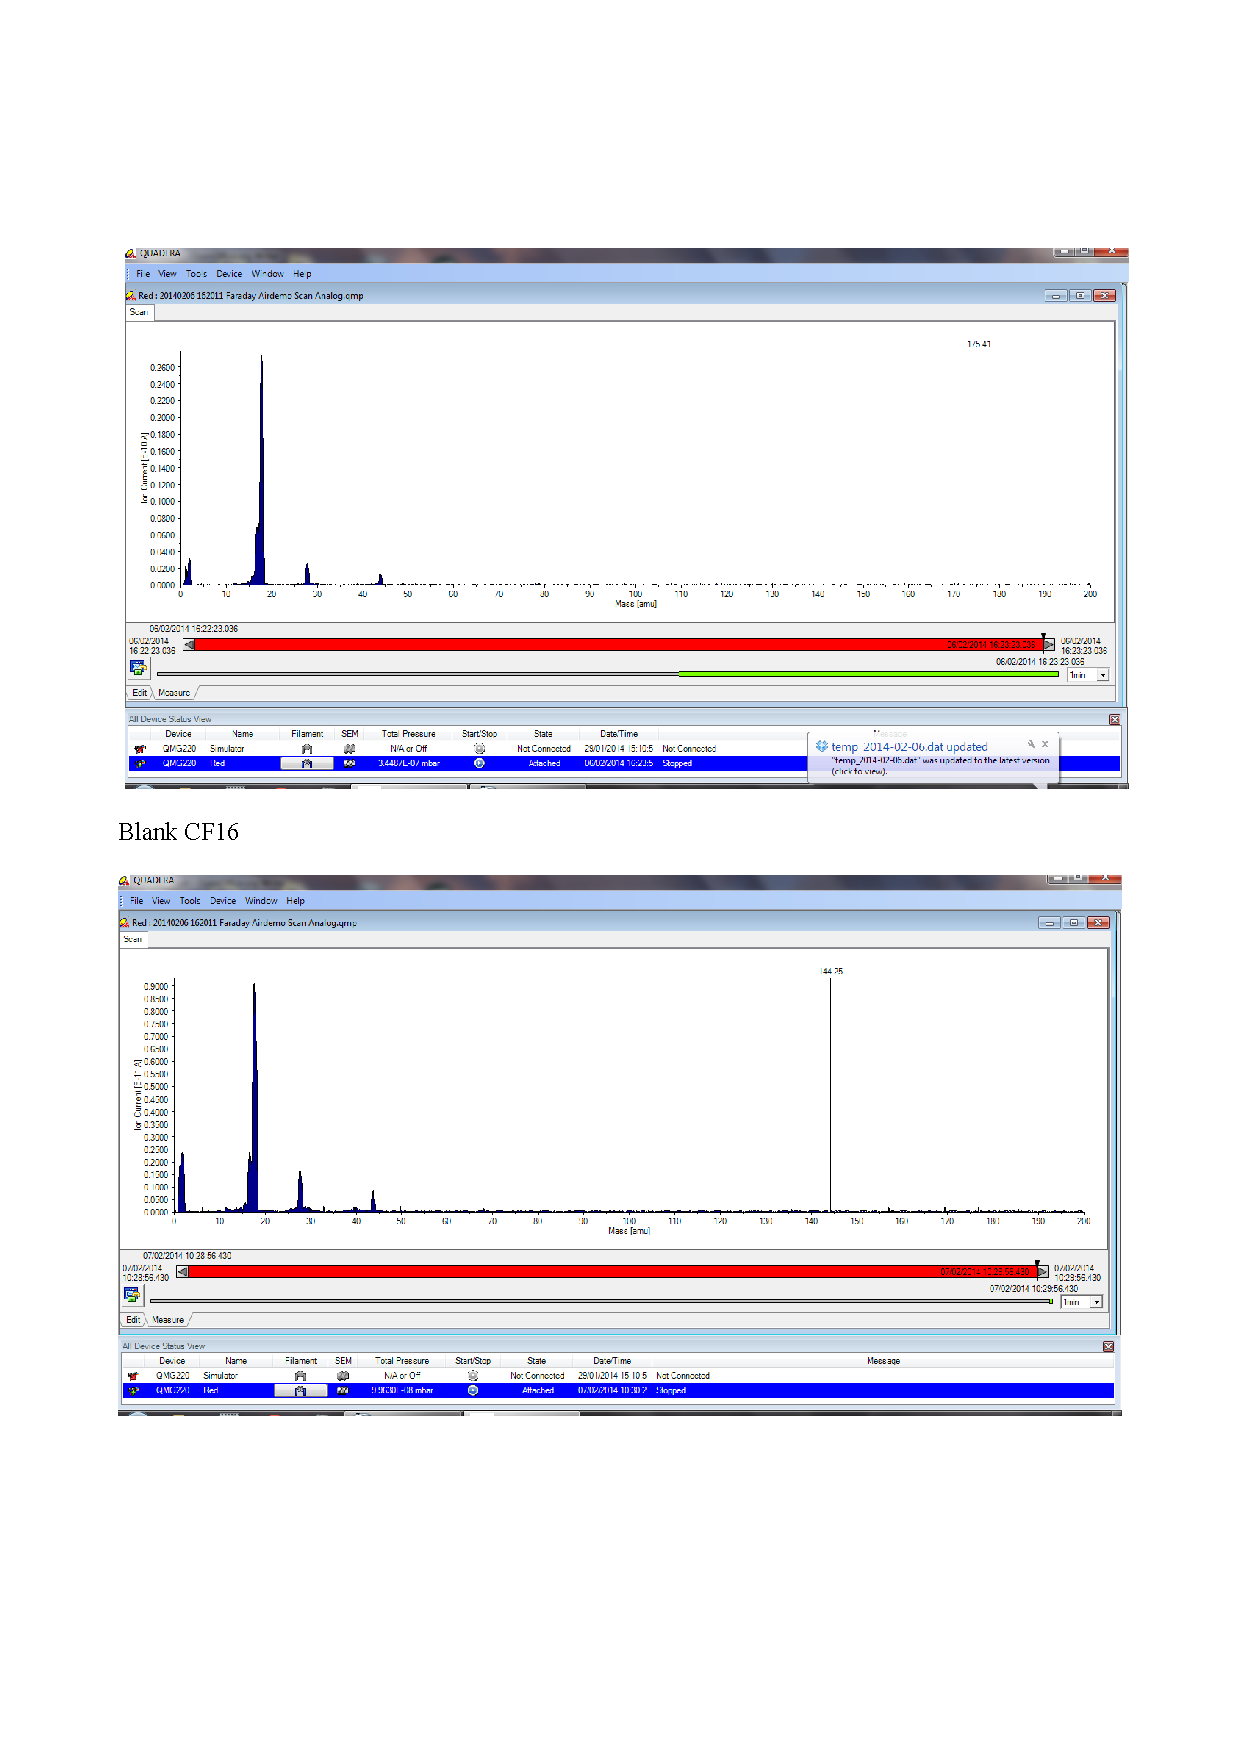
\includegraphics[width=0.65\textwidth,height=0.55\textwidth]{img/Opt_Gel_1}
  \end{center}
  \caption{RGA mesurement of NyoGel OCK-451 compared to a blank RGA.}
  \label{fig:gelRGA}
\end{figure}
\begin{figure}
  \begin{center}
    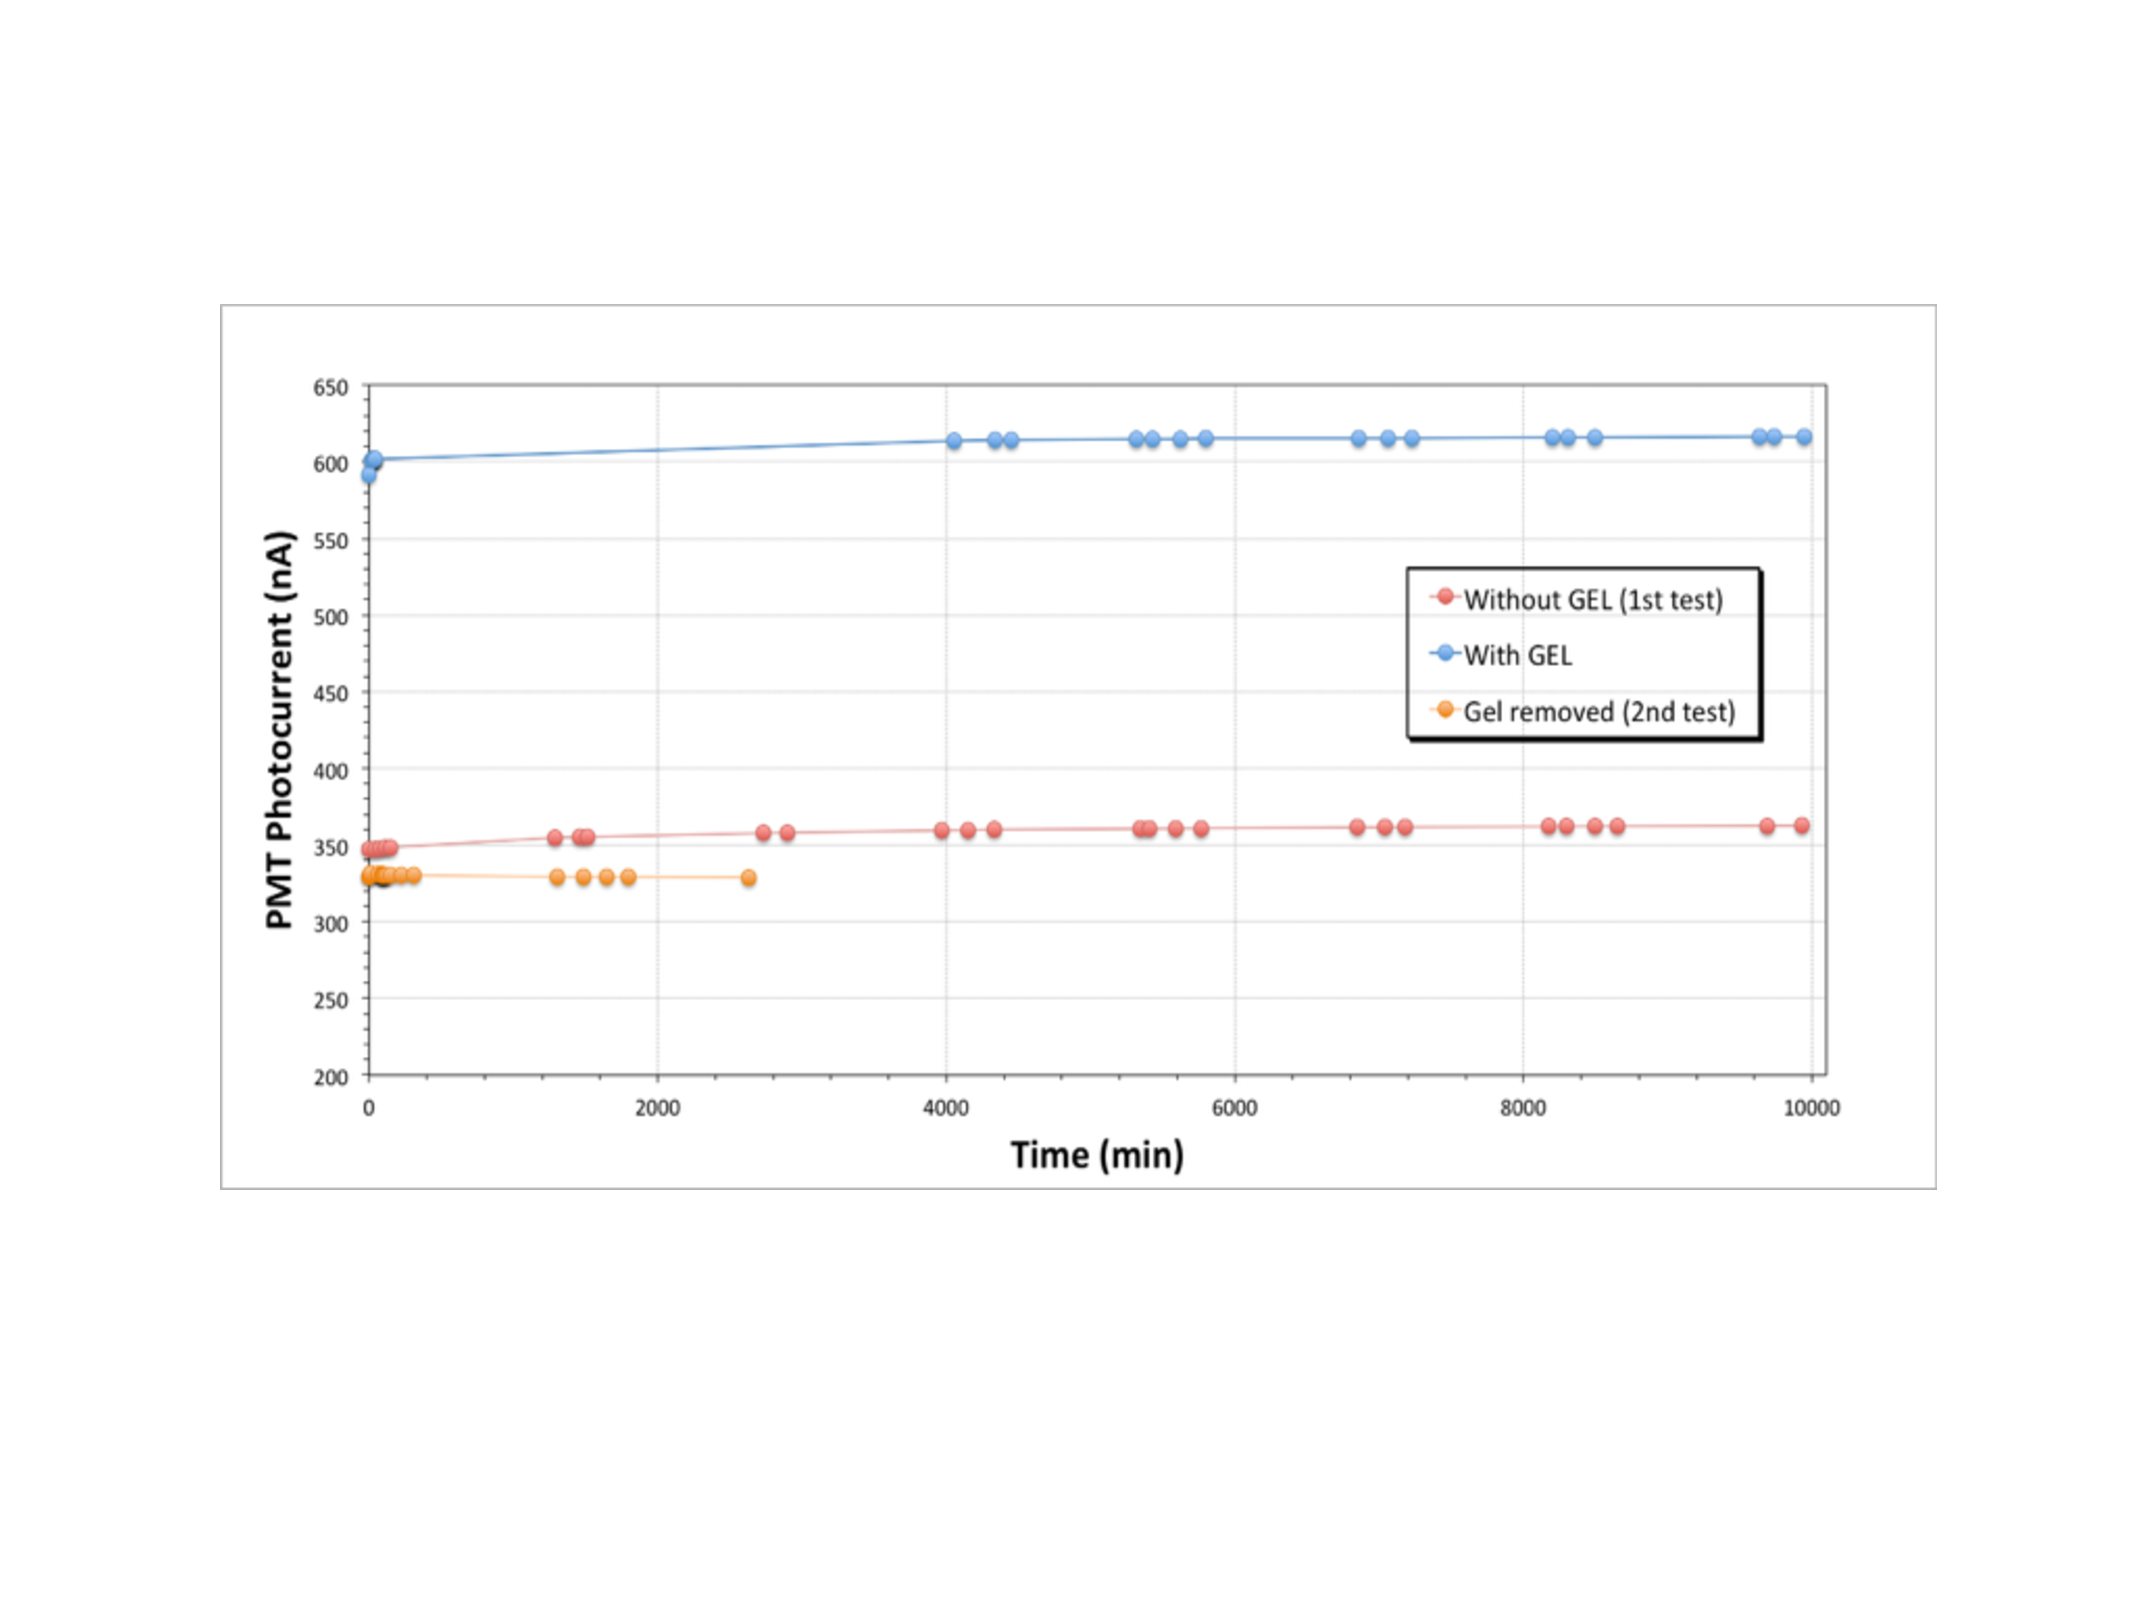
\includegraphics[width=0.65\textwidth]{img/gelPlot}
  \end{center}
  \caption{PMT photocurrent for pulses of calibrated LED with
    time. Curves compare the current in vacuum with the PMT behind a
    sapphire window with and without an optical coupling gel (NyoGel~OCK-451).}
  \label{fig:gelPer}
\end{figure}

\subsection*{Proposed aims of the project}
\label{subSec:Prop}
The proposal will involve the extension and formalisation of the work
currently undertaken by the PI. He will continue to coordinate the
development and construction of the Energy plane of NEW and will
update and develop the run coordination protocols for application to
data taking at LSC. Moreover, he will
generalise his work on detector calibration to involve all aspects of
the calibration of the detector energy measurement, optimising
techniques used in DEMO and developing others to meet the challenges
of the larger scale detectors. Additionally, he will begin R\&D using
NEXT-DEMO for a potential upgrade using next-generation SiPMs as both tracking and
energy measurement sensors.

\subsubsection*{Coordination of NEW energy plane construction}
The main mechanical and electronic designes for the energy plane of
NEW are already decided and under construction. The PI will continue
as the coordinator ensuring the the efficient marriage of all sections
of the energy plane and their integration with the other sections of
the detector.

NEW and, particularly the energy plane group, has reached the
construction stage and the role of the coordinator has become even
more important. He will be required to coordinate the arrival of the
pieces which have already been sent for construction, their testing
under pressure and vacuum conditions, their cleaning to eliminate
surface radioisotope contamination and the construction and
integration of all components (main components shown in figure \ref{fig:EPlane}). Additionally, the optical gel must
undergo radiopurity testing invloving the definition of the
methodology to be used for its application to ensure that the
measurement best represents the material to be used. The PI will work
directly with the mechanical, electronic and radiopurity experts to
ensure the efficient completion of all tasks.
\begin{figure}
  \begin{center}
    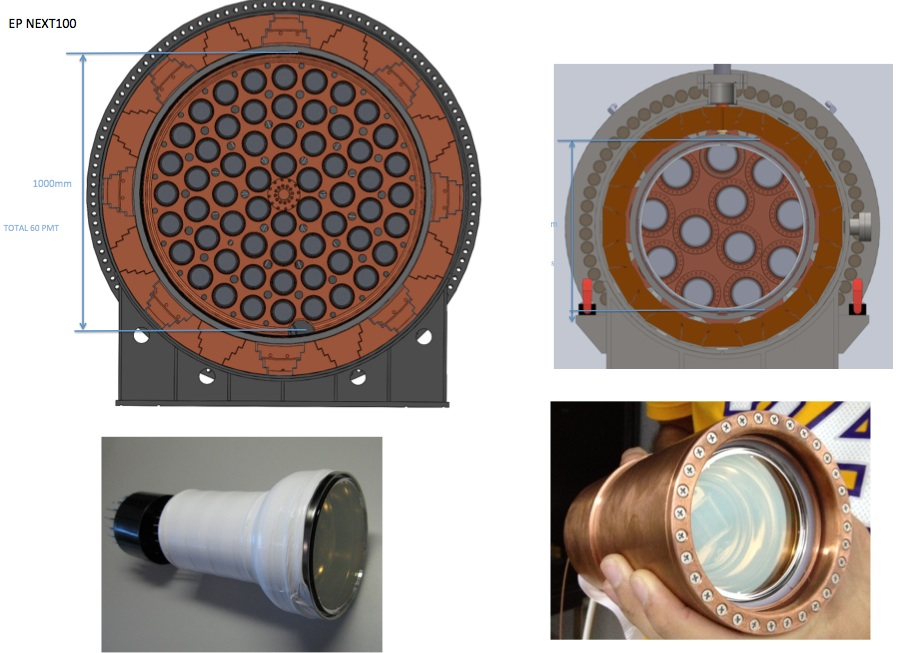
\includegraphics[width=0.65\textwidth]{img/EP.jpg}
  \end{center}
  \caption{Major energy plane components of NEW and NEXT-100.}
  \label{fig:EPlane}
\end{figure}
A prototype PMT vacuum can has been tested at IFIC with an appropriate
material having been chosen (silver braze) because of its radiopurity and the
bond made by brazing the sapphire window to the copper can using this
material being
robust against relative pressures of 20~bar. The mass production of
the half cans which will be used to seal the energy plane support
plate against pressure will be supervised by the PI. The proceedure
will involve:
\begin{itemize}
\item Arrival of half can copper structure to IFIC.
\item Arrival of sapphire windows to IFIC.
\item Sending of both components to Morgan Advanced Materials in the UK for brazing.
\item Testing of the 12 complete half cans under pressure.
\item 'Dirty' testing of energy plane components at IFIC.
\item Sending of half cans for cleaning and TPB coating at Gran Sasso.
\item Receipt of cans at LSC.
\end{itemize}
Additionally, the energy plane support plate will also be sent to Gran
Sasso for cleaning and will subsequently be sent to
LSC. Simultaneously, the 12 PMTs to be used in NEW will be selected by
having their absolute gain and QE determined and those with similar
values grouped together. All components will then be sent to LSC for
integration with the mechanical components arriving from Gran Sasso.

As much of the cleaning of the components will take place at LSC and Gran Sasso
laboratory in Italy, the PI will coordinate with the facilities to
organise the delivery of each item to the appropriate place for
cleaning and, ultimately, to LSC for integration with the other
detector components.

\subsubsection*{Run coordination}
The NEXT-DEMO run coordination, shift scheduling and data monitoring
protocol has served as a small scale test of the protocols which will
be implemented to ensure that the data taking of both NEW and NEXT-100
runs smoothly. The basic requirements for the implementation of this
protocol are the following:
\begin{itemize}
\item Coordination with the system managers of the experiment and LSC
  to determine the optimum positioning of the detector slow control
  monitors and the shifter areas both inside the laboratory and inside
  the office buildings.
\item Coordination with individual detector component experts for the
  writing of documentation.
\item Coordination with laboratory safety to determine proper
  proceedures required for shifters.
\item coordination with software and data experts to ensure proper
  data monitoring infrastructure available before data taking begins.
\end{itemize}
Currently, it is expected that the run coordination and scheduling
will take the following format:
\begin{itemize}
\item Three shifts per day for detector supervision (initial phase).
\item Experts on call (initial phase).
\item Weekly coordination meeting for review of week and scheduling of
  calibrations and maintenance and change of shift.
\end{itemize}

\subsubsection*{Calibration}
The calibration aims proposed are more general than those performed in
DEMO. The initial deliverable in NEW will be the definition of the LED
settings for the PMT calibration. NEW will have multiple available
LEDs and is, of course, much larger than DEMO. The studies will
optimise the calibration of the PMTs both using individual PMTs and
the array as a whole so that the response of the PMTs can be
understood and any position dependency in the calibration limited.

The more general calibration protocol of the detector will involve the
use of multiple radioactive sources. Determination of the variation of
response to X-ray deposits must be understood in general as a first
step. The PI will begin by optimising the methods published
in\footcite{Lorca:2014sra} using DEMO data and will then work with the rest of the
calibraiton group to study the required data and its best application
within the optimised code to determine the drift and detector
correction factors to correct the response and to calculate the energy
scale. This deliverable will also require interaction with simulation
groups so that the methodology is fully understood and its systematic
errors accurately estimated.

\subsubsection*{R\&D with DEMO}
In addition to the aims concerned with the development and
exploitation of NEW and NEXT-100 the PI will undertake an innovative
new project to test the posibility of replacing the the PMTs of the
energy plane with next-generation SiPMs with very low dark current and
noise.

SiPM technology has developed a great deal since the beginning of the
NEXt project. The current generation of sensors from SensL
technologies for example have dark currents as low as 70~kHz (compared
to 400~kHz for the models which have been sed in the NEXT-DEMO
tracking plane). This coupled
with improved electronics, the lower mass of material for the same
coverage when compared to PMTs and higher radiopurity of
the materials used in their construction make SiPMs an attractive
technology for use in low background experiments like NEXT.
\begin{figure}
  \begin{center}
    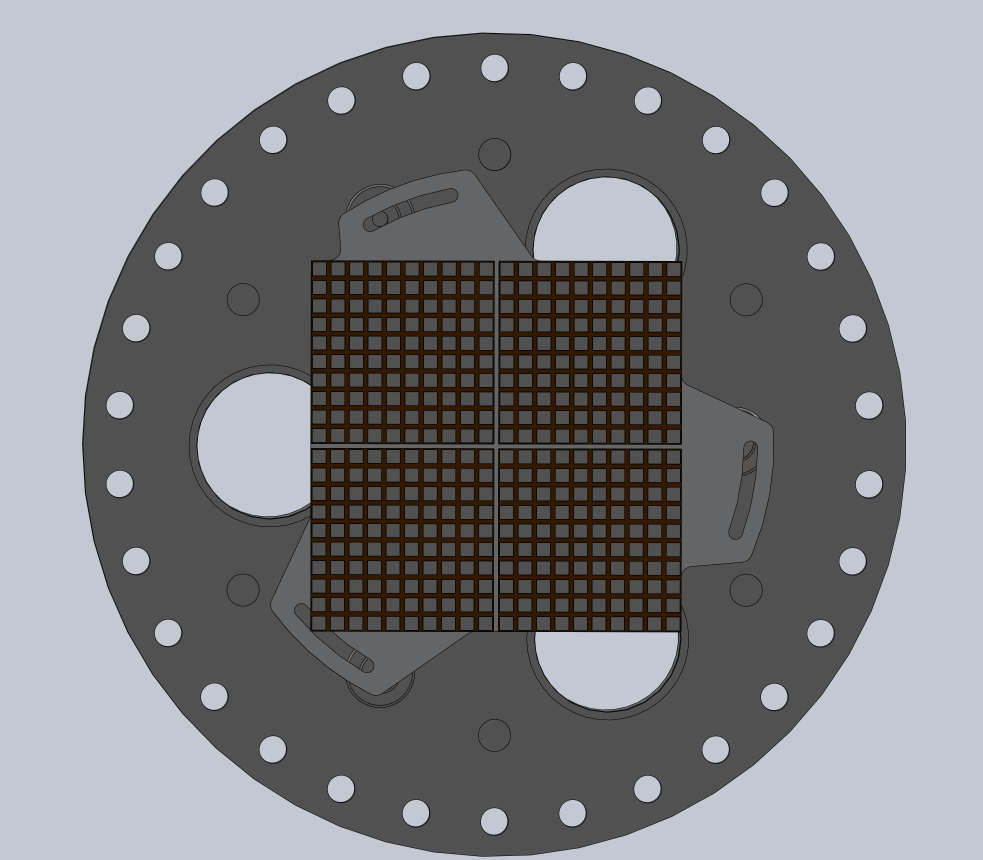
\includegraphics[width=0.495\textwidth]{img/siliEng}
    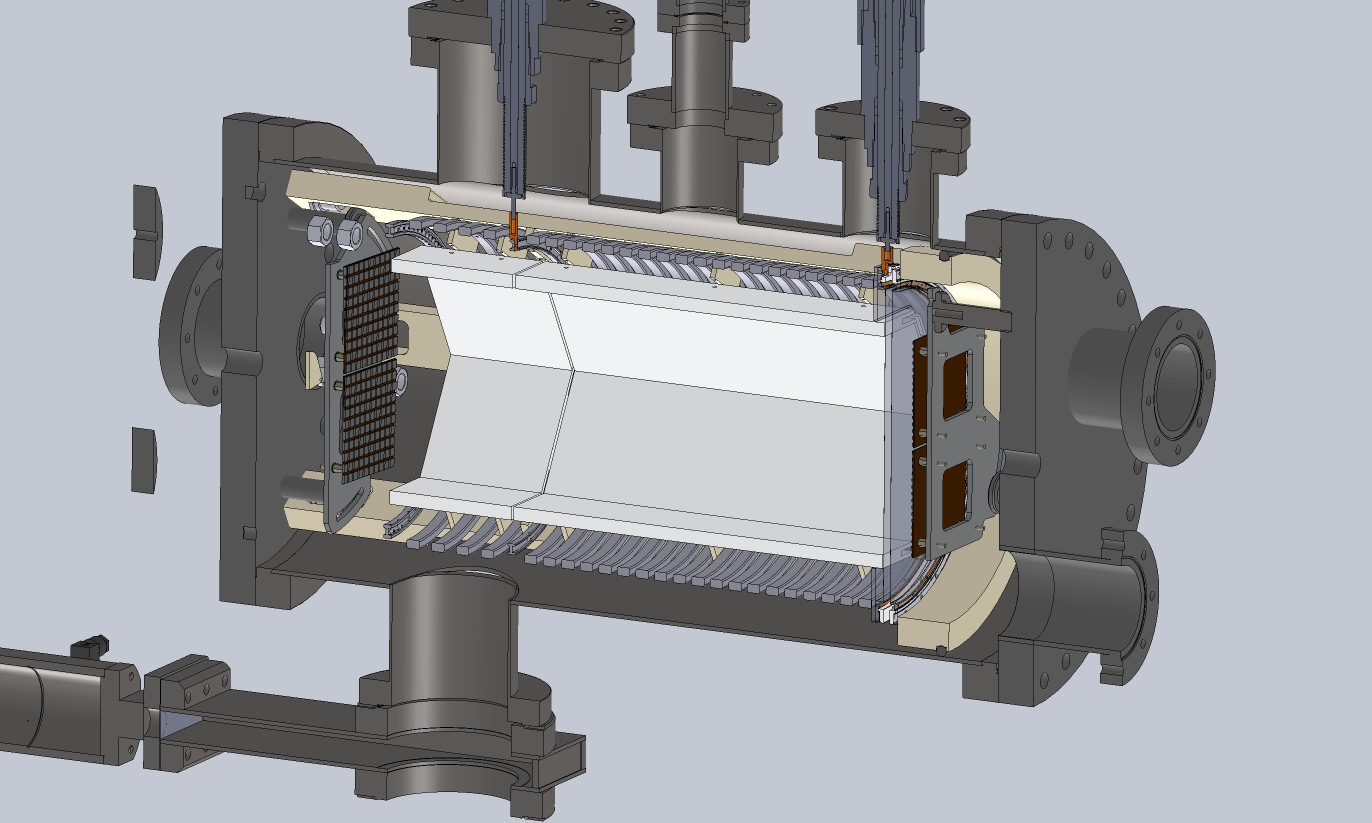
\includegraphics[width=0.495\textwidth]{img/siliNEXT}
  \end{center}
  \caption{The proposed SiPM energy plane for R\&D with NEXT-DEMO.}
  \label{fig:siliNEXT}
\end{figure}
Another possible advantage of the use of SiPMs without the need for
PMTs is the attractive possibility to apply a magnetic field to the
detector (PMTs do not function correctly in a magnetic field and would
distort the field lines). With, for example, roughly solenoidal field
lines runing parallel to the drift direction in the TPC transverse
diffusion of the charge cloud would be redused, improving x/y position
reconstruction resolution. Moreover, the electrons depositing energy within
the gas would be forced into helical paths which would reduce the
dominance of multiple scattering and open up the possibility to look
for curvature changes in tracks indicative of double electrons. These
improvements could help to further reduce the background to \bbonu\
event s from natural radiation in a future tonne scale NEXT.

The project will involve the design and building of a new energy plane
made of a tightly packed array of SensL 6$\times$6~mm$^2$ SiPMs,
coating with TPB and installation in NEXT-DEMO followed by its commissioning and the determination
of its sensitivity. The two most pressing measurements are:
\begin{enumerate}
  \item Determination of energy resolution using SiPM: calculations
    show that the new sensors should be able to achieve signal to
    noise levels of ~35 at \Qbb.
  \item Determination of scintillation (t0) signal detection
    efficiency. Signal to noise at the light levels expected is still
    low but cooling of the gas is an option which could improve the
    efficiency.
\end{enumerate}
% Part of the PI's time would be spent on the construction and
% characterisation of the the new SiPMs and their integration into DEMO
% and, ultimately, in the demonstration of the efficient detection of
% the primary scintillation signal and of the possible energy resolution
% achievable.

\subsection*{Match to the National Programme for research aimed at the
  Challenges of Society}
This research project is presented within the program of ``Challenges of society'', specifically, challenge number 6: {\bf Change and social innovation.}

We argue that this project represents a major innovation in the way that particle physics is conducted in Spain, and thus marks a path to a more productive approach to research.

Particle physics is a clear example of so-called ``big science''. The discovery of the Higgs boson is a quintessential example of such big science. It has required the construction and operation of the LHC, one of the most impressive scientific machines ever built by humankind. The gargantuan scale of the effort could only be faced by a collective effort centralised at CERN, the largest particle physics laboratory in the world.  

Big science involves big budgets, often invested in purchasing equipment to be installed at CERN and in paying scientific staff whose activity also develops at CERN. Such large budgets are often justified in terms of industrial and scientific returns. While those returns certainly exist, {\bf they tend to be larger for countries who are already well developed scientifically}. Specifically, the positions of leadership in the large CERN experiments, and in the CERN scientific and technical divisions, are dominated by countries like Germany, Switzerland, U.K., France and Italy. 

Remarkably, the countries leading the big science at CERN and other
laboratories have also developed ``national science'' physics
programs. A case of great interest is Italy, a country not very
different from Spain, in terms of GDP and social habits. However, the
international impact and the returns of physics in Italy are much
larger than in Spain. For example, the number of Spanish staff members
at CERN is 115, to be compared with 275 for Italy (which has the
second largest staff population, after France, who co-hosts the
lab). Adding fellows and associates (that is, temporary CERN
contracts, often given to scientists), the figures for Spain are 363,
to be compared with 1726 for Italy\footcite{cernstats}. Several
Italians have served as CERN general directors, and have led or are
leading the LHC experiments. There is also a high probability that
Fabiola Gianotti (another Italian) will become director. Moreover, Italy has five Nobel prizes in physics (Marconi, 1909, Fermi, 1938, Segrè 1959, Rubbia 1984, Giacconi 2002), while Spain has none. 

Remarkably Italy also boasts the best underground laboratory of
Europe, and one of the best of the world, the LNGS (Gran Sasso). The lab hosts 20 experiments including three searching for \bbonu\ processes (GERDA, CUORE and COBRA) and two experiments searching for Dark Matter (WARP and XENON). 

Through these experiments, Italian physics {\bf attracts external talent} (some of the best physicists from Europe and the USA participate in experiments at the LNGS) {\bf and external funding}, complementing the big science at CERN with physics on a smaller scale concerning human resources and budgets. However, such ``local'' physics results in discoveries of great scientific impact (such as the discovery of neutrino oscillations, which has been the result of a world-wide effort involving underground laboratories in Italy, USA, Canada, Russia and Japan). It also allows the training of students and post-docs in experiments where young physicists can make a major impact at all levels, ranging from the construction of the detector to the analysis of the data. Last, but not least, such local science has an important impact in the Italian industry and in the appreciation of science by the public in general. 

{\bf We argue that, in order to balance and optimise the current big science effort in Spain, it is necessary to develop the physics at the LSC, in analogy to the Italian case.} NEXT is the flagship experiment of our national laboratory, and has achieved international recognition, as demonstrated by the fact that NEXT is a recognised CERN experiment and has obtained an AdG/ERC, {\bf the first grant of this type in Spain in the field of experimental particle physics}. 

We, therefore, consider that the NEXT project is a clear example of social innovation, as it has the potential of implementing profound changes in Spanish science. As described in this project, NEXT, through its various stages, can make a major discovery. It will bring international credit and visibility to our science and to the LSC. %And it has an important impact both in local industry (through contracts to many national firms, and development of high technology) and in the public perception of science. 

%Furthermore, the on-going collaboration with the CLPU further reinforces the above arguments, since the effort involves now a second national scientific installation. In addition, the \BATA\ program implies a major example of interdisciplinarity, and can result in a number of important technological returns (development of infra-red laser technology, which has a myriad of scientific and technological applications).

Finally it is important to remark that, while the usual operation of
big science in Spain implies to finance the participation of our
groups (including the annual CERN quota, the common fund of the
experiments and the contributions to construction and operation of the
CERN experiments), the national science that NEXT represents obtains
external funding through ERC projects (including the AdG and several
H2020 actions currently in progress involving LSC), as well as the
contributions of the international collaboration to detector
construction and operation (in particular, in the case of NEXT through
the USA groups led by Prof. David Nygren, the inventor of the
technology on which NEXT is based). NEXT also attracts external talent
to our country, as the intense collaboration with top USA universities
demonstrates. The PI himself is originally from the UK where he
undetook his studies, has worked in Japan and was attracted back to
Europe and to Spain by the scientific potential of NEXT and the
quality of scientists both at IFIC and in the wider collaboration.

%Last but not least, the NEXT experiment (and in particular the
%collaboration with the CLPU) involves the extensive development of
%photonics, listed as one of the  ``Facilitating Essential
%Technologies''.

\subsection*{Timetable and costing}

\subsubsection*{Specific objectives}
The objectives concerned with the project description above are as
follows:
\begin{enumerate}
  \item Construction and testing of the PMT half cans; expected
    delivery during first quartile 2015 (Q1'15).
  \item Basic calibration of the PMTs; expected
    delivery during of first quartile 2015 (Q1'15).
  \item Pressure testing and dirty construction at IFIC (Q1'15).
  \item Cleaning and delivery to LSC (Q2'15).
  \item Installation of NEW at LSC (Q2'15).
  \item Definition of run coordination protocol (Q2'15)
  \item Optimisation of energy plane and X-Ray calibration methods
    (Q4'14-Q2'15).
  \item Implementation of calibration working with wider calibration
    group (Q3'15).
  \item Acting as run coordinator for the NEW data runs (Q1-Q4'16).
  \item SiPM energy plane Construction (Q2'15)
  \item SiPM energy measurement R\&D phase (Q3'15-Q1'16).
  \item NEXT-100 energy plane component construction (Q1-Q4'16)
  \item NEXT-100 installation at LSC (Q1'17).
  \item NEXT-100 eng plane commissioning (Q2-Q4'17).
\end{enumerate}

\subsubsection*{Specific budgetary requests}
In addition to the PIs salary the project requests cover for visits to
Grans Sasso and for stays at LSC for meetings and the construction and
commissioning phases, cover for conference attendance and
funding for the SiPMs and related electronics for the R\&D
deliverable. A specific costing of these requests can be found in
table \ref{tab:TCOSTS}.
\begin{table}[!h]
  \begin{center}
    \begin{tabular}{|l|r|}
      \hline
      Item              & Total Cost \euro  \\
      \hline
      Travel to Gran Sasso & \\
      Stays at LSC & \\
      1 Conference per year & \\
      1000 SensL SiPMs & 23000 \\
      Kapton boards for new eng plane & \\
      \hline
      Total  NEXT        &  \\
      \hline
    \end{tabular}  
    \caption{Total costs of the project.}
    \label{tab:TCOSTS}
  \end{center}
\end{table} 

\noindent\textbf{C.2. IMPACTO ESPERADO DE LOS RESULTADOS}\\


\noindent\textbf{C.3. IMPLICACIONES \'ETICAS Y/O DE BIOSEGURIDAD}\\
The proposal involves no ethical nor biosecurity implications.

\end{document}